\subsection{Geometrical analysis of feature trajectories}
\label{sec:geometrical_analysis}

In this section we analyze the geometry of the trajectories regarding the weight-tied convnext vs the standard convnext.
We also compare the standard convnext with resnet and swin, whose properties are very similar since they are non weight-tied and
the network learned to make the blocks perform an unique functionality of one step, so there is no reason for the network to learn a more
complex dynamic.

\subsubsection{Massive activations excluded from analysis}
\label{sec:massive_activations}

After analyzing some trajectories on our first aproach, they seemed too homogeneos in convnext and swin cases, so we analyzed the features and
founded the so called massive activations \cite{sun2024massiveactivationslargelanguage}. In convnext shared and non-shared there is one channel that grows indifinetly.
We did a similar analysis and concluded the same as \cite{sun2024massiveactivationslargelanguage}

\subsubsection{Trajectories of weight-tied convnxt vs standard convnext}


\subsubsection{Trajectory analysis of weight-tied convnext}
\label{sec:refinement_error}
Inpired by some of the metrics of \cite{pandey2026trajectorygeometrytransformerrepresentations} we perform an analysis of the trajectories
ignoring the massive channels of Convnext and the massive tokens of swin. Resnet does not show signs of massive activations.

In weight-tied convnext we can see in Figure \ref{fig:teaser} right the norm of the velocity, that is $f(x(t))$ that has a shape of a bell curve.
This information only shows if the point is moving or not, but it doesn't tell if it rotates or move towards the same direction.
That's why we plot several new metrics:

\textbf{Acceleration}

Here we decompose the acceleration vector into the sum of two components: The tangential and normal accelerations with respect to the velocity.
Note, that in a high-dimentional space of 300,000 dimensions (the case of Stage 3 in convnext), there are 299.999 dimentions that are normal with the velocity, and only 1 that is tangent.
The tangent component can be negative or positive with respect to the velocity that is, it reduces or increases the current velocity in this 1D line, but we cna only analyze the norm of the normal acceleration.
Even in a such space, that tangential acceleration has a big representation.

We can see

\textbf{Angular acceleration}
\textbf{Trajectory curvature}

\textbf{The shape of the trajectory}

With all this tools, we conclude that the trajectory at the start rotates at high speeds, giving the trajectory a high curvature,
but with low velocity norm, that implies that it does small steps changing constantly of direction. The model is computing the direction where it has to accelerate the point to.

After that, the model starts to accelerate towards one direction, angular speed decreases, norm of angular acceleration increases due to the reduction of velocity
the result is a major reduction on the curvature of the trajectory, while tangential acceleration hits its maximum. The model is expanding the most important features.

Finally, angular acceleration decreases, tangential acceleration rapidly decreases, becoming negative, the velocity decreases, the angular velocity increases again, and curvature raises again. We have the same
scenario as in the first phase. The model is refining features again.

We observe that for the 500 images we analyzed, the trajectory is mostly of this form. But in the variance analysis,
the velocity has its maximum variance on the second phase since the model is pushing the features of different classes apart from the origin in different directions.

\subsubsection{Refinement error: accumulated vs.\ bounded}
\label{sec:refinement_error}

\begin{figure*}[t]
    \centering
    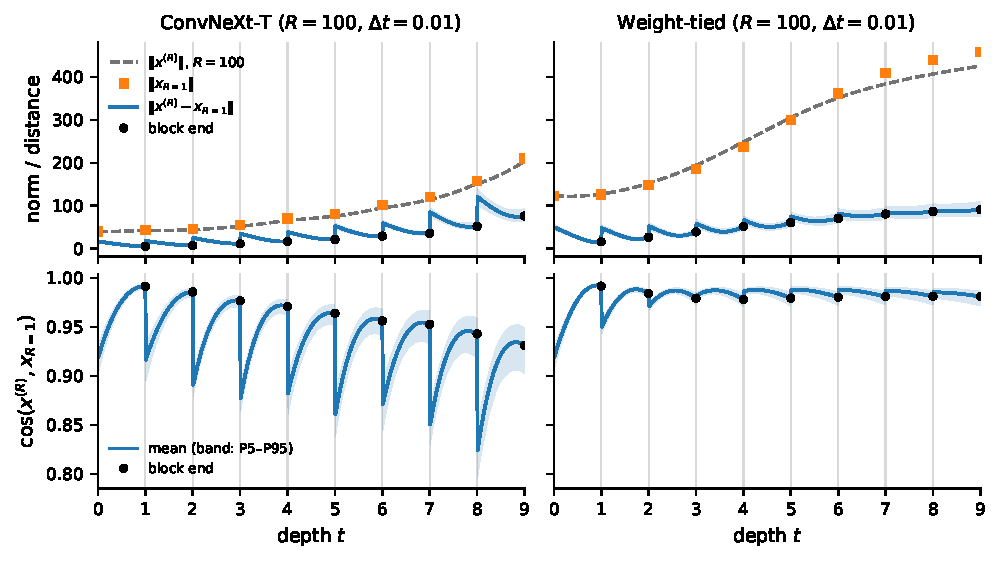
\includegraphics[width=\textwidth]{figures/dist_cos_r1_compare.pdf}
    \caption{Refined vs.\ native ($R{=}1$) stage-3 path for the standard (left) and
    weight-tied (right) ConvNeXt-T.
    \textbf{Top:} $\|x^{(R)}-x_{R{=}1}\|$ (solid) with both state norms for scale
    (dashed: refined; squares: native).
    \textbf{Bottom:} $\cos(x^{(R)},x_{R{=}1})$.
    Mean and P5--P95 over the same 500 images; massive channel ignored; dots mark the end
    of each native step.
    The switched stack accumulates angle at every block; the shared field saturates.}
    \label{fig:dist-r1-compare}
\end{figure*}

\Cref{fig:dist-r1-compare} repeats the comparison of \cref{fig:dist-r1} for the
weight-tied network.
Both models start the same way: after the first native step the cosine to the $R{=}1$
path is $0.99$.
They then diverge.
In the standard ConvNeXt-T the block-end cosine keeps falling, to $0.93$ at $t{=}9$:
each block receives an input that has already drifted and adds its own discretisation
error on top.
In the weight-tied model it settles at $\approx 0.98$ after two or three steps and stays
there for the rest of the stage, so a single autonomous field keeps the refinement error
bounded instead of accumulating it.
The norms also behave differently: in ConvNeXt-T they nearly coincide ($203$ vs.\ $210$),
whereas the weight-tied refined path ends about $7\%$ shorter ($427$ vs.\ $458$), so part
of its smaller gap is radial.
% TODO: relate the bounded error to the contractivity of the shared field.

\subsubsection{Integrating beyond the trained horizon}
\label{sec:beyond_horizon}
% TODO: constant velocity regime: f(x) saturates, x grows along a fixed direction for T >> n.
There is big difference between weight-tied convnext and standard convnext: First one reaches a velocity plateau
where the input just grows indifinetly in the same direction.

In standard convnext, swin and resnet are different, we used R=100 with euler step 1,
since the blocks use different parameters and the network was not trained to reuse params,
it has a similar dynamics as the R=100 with Euler step of 0.01 but with more magnitude.
